\documentclass[UTF8,a4paper]{article}
\usepackage{ctex}
\usepackage[utf8]{inputenc}
\usepackage{amsmath}
\usepackage{pdfpages}
\usepackage{graphicx}
\usepackage{wrapfig}
\usepackage{listings}
\usepackage{multicol}
\newcommand{\tabincell}[2]{\begin{tabular}{@{}#1@{}}#2\end{tabular}}
\title{实验三\ \ 负反馈电路仿真及实验}
\author{张蔚桐\ 2015011493\ 自55}
\begin {document}
\maketitle
\section{预习任务}
\subsection{两级放大电路的恢复性调试}
这里我们回顾一下两级放大电路在仿真和实验中的性能指标

\begin{table}
\centering
\caption{两级放大电路在仿真和实验中的性能指标}
\begin{tabular}{|c|c|c|c|}
\hline 
测试情况 & 放大倍数$A_u$ & 输入电阻$R_i$ & 输出电阻$R_o$\\
\hline 
仿真 & -168 & $91\mathrm{k}\Omega$ & $3.08\mathrm{k}\Omega$ \\
\hline 
实际电路 & -155 & $91.6\mathrm{k}\Omega$ & $3.08\mathrm{k}\Omega$ \\
\hline 
\end{tabular}
\end{table}
\subsection{两级放大电路电压并联负反馈电路的设计}
\begin {wrapfigure}{r}{0pt}
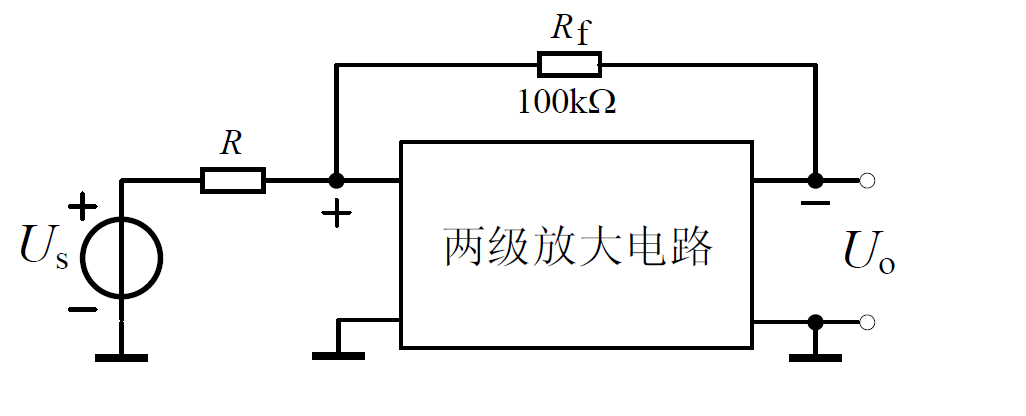
\includegraphics [width=60mm]{circuit.png}
\caption{实验用电路图}
\label{Circ}
\end {wrapfigure}
如图\ref{Circ}所示是实验用电路图,首先进行理论计算

若电路引入深度负反馈,则有
$$ A_{usf}\approx \frac{1}{FR}=-\frac{R_f}{R}=-10$$
可以立即解得$R=-\frac{R_f}{A_{usf}}=10\mathrm{k}\Omega$

同时计算深度负反馈条件得到
$$1+A_uF=1+A_u\frac{R_i}{R_f}\approx154 >>1$$

满足负反馈条件

同时进一步有,因为引入电压并联负反馈,输入电阻减小为
$$R_{if}=\frac{R_i}{1+AF}=591\Omega$$
输出电阻减小为
$$R_{of}=\frac{R_o}{1+AF}=20\Omega$$
\subsection{仿真测试}
仿真按照设计的要求完成电路的设计,得到的电路如图\ref{ACT}所示,相关的静态工作点已经标注在图中,我们得到$I_{CQ}=I_{DQ}=2\mathrm{mA}$,同时得到

\begin{figure}
\centering
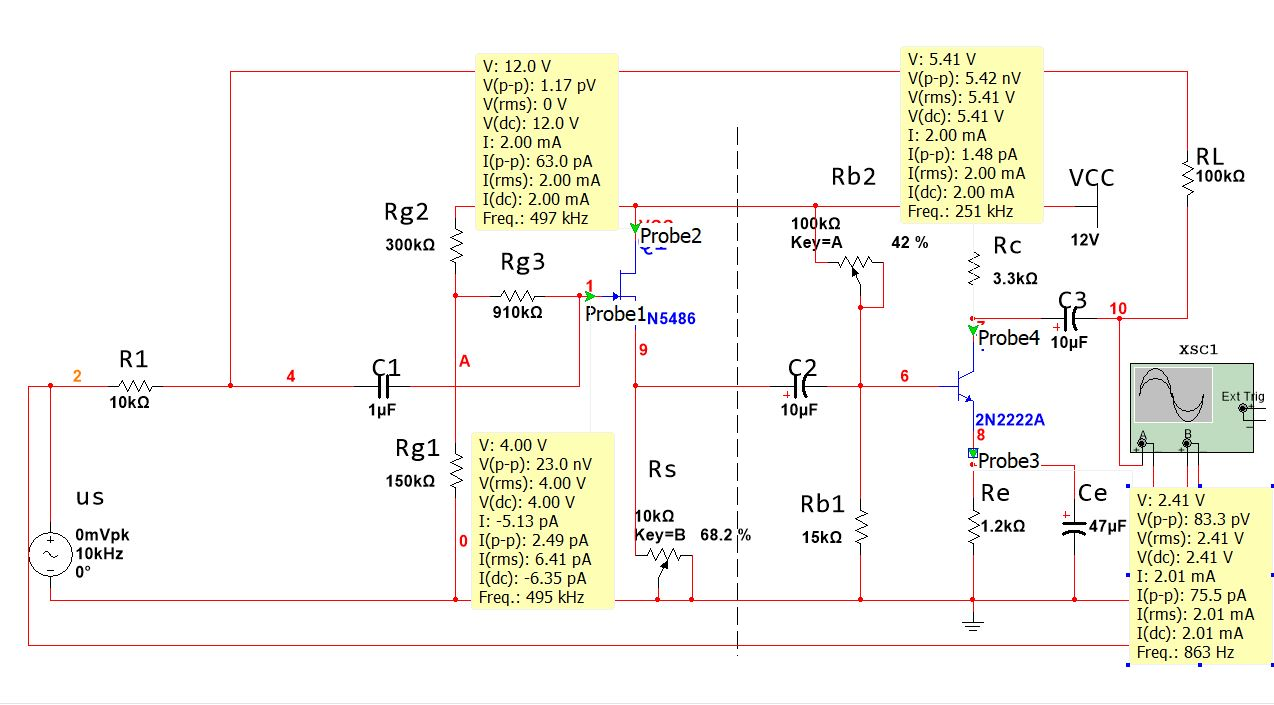
\includegraphics[width=\textwidth]{cir.jpg}
\caption{实验电路}
\label{ACT}
\end{figure}
\begin{figure}
\centering
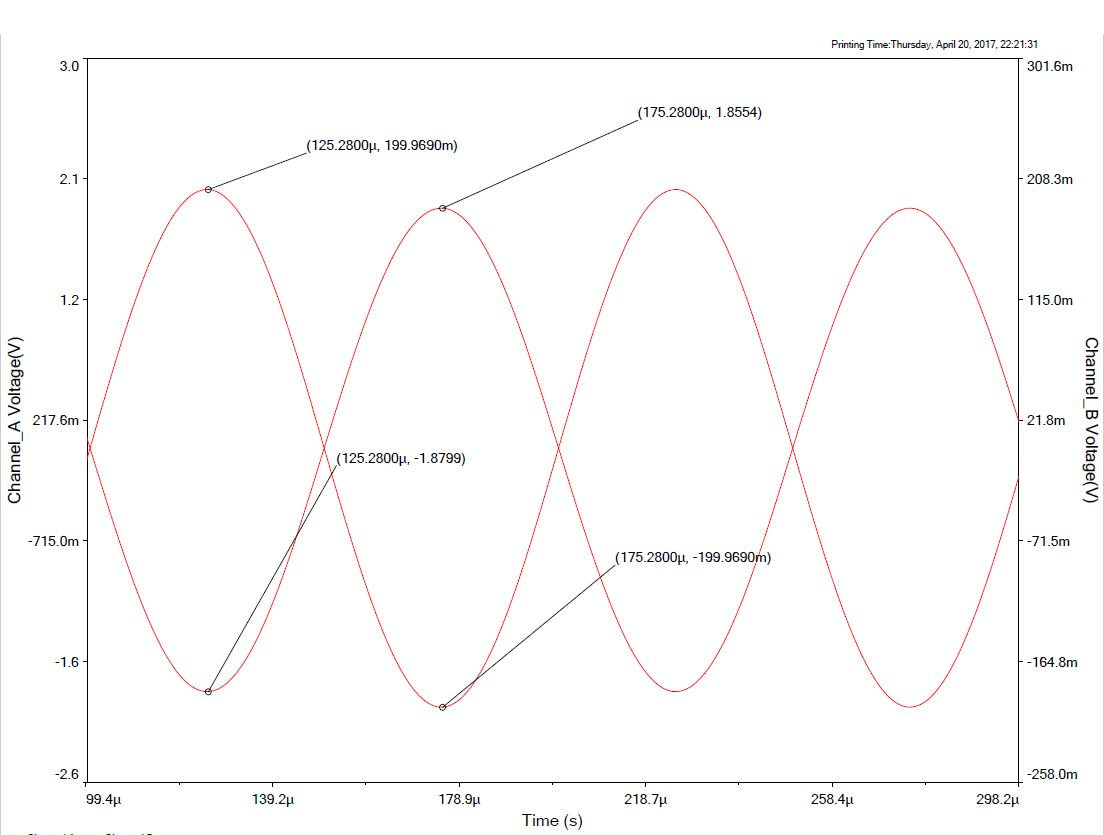
\includegraphics[width=\textwidth]{A.jpg}
\caption{负载开路放大倍数测试}
\label{A}
\end{figure}
所示,相关的静态工作点已经标注在图中,我们得到$I_{CQ}=I_{DQ}=2\mathrm{mA},U_{GDQ}=-8\mathrm{V},U_{CEQ}=3\mathrm{V}$满足题目中给定的要求

进一步按照题目中设置信号源幅度为200mV,频率为10kHz,得到电压放大倍数为如图\ref{A}所示,并且得到
$$A_{usf}=-\frac{1878.9+1855.4}{199.97+199.96}=-9.34\approx -10$$
和题目要求相近,同时测得负载开路输出电压峰峰值为$U_{o0}\approx1866\mathrm{mV}$

同时采用串联电阻法测量输入电阻,如图\ref{R}所示,可以计算得到输入电阻为
$$R_i=\frac{28.5\mathrm{mV}}{37.1\mu\mathrm{A}}=768\Omega$$
输出电阻为$$R_o=\frac{1878.9+1855.4-3680\mathrm{mV}}{368\mu\mathrm{A}}=147\Omega$$
同时,在$10\mathrm{k}\Omega$负载电阻下$A_{usf}=-9.2$基本的变化趋势和理论估算的是一致的。

同时可以得到辐频特性曲线如图\ref{F}所示。可以看出低频截止频率约为17Hz,高频截止频率约为9.6MHz,但是在4MHz以上已经不稳定。

\begin{figure}
\centering
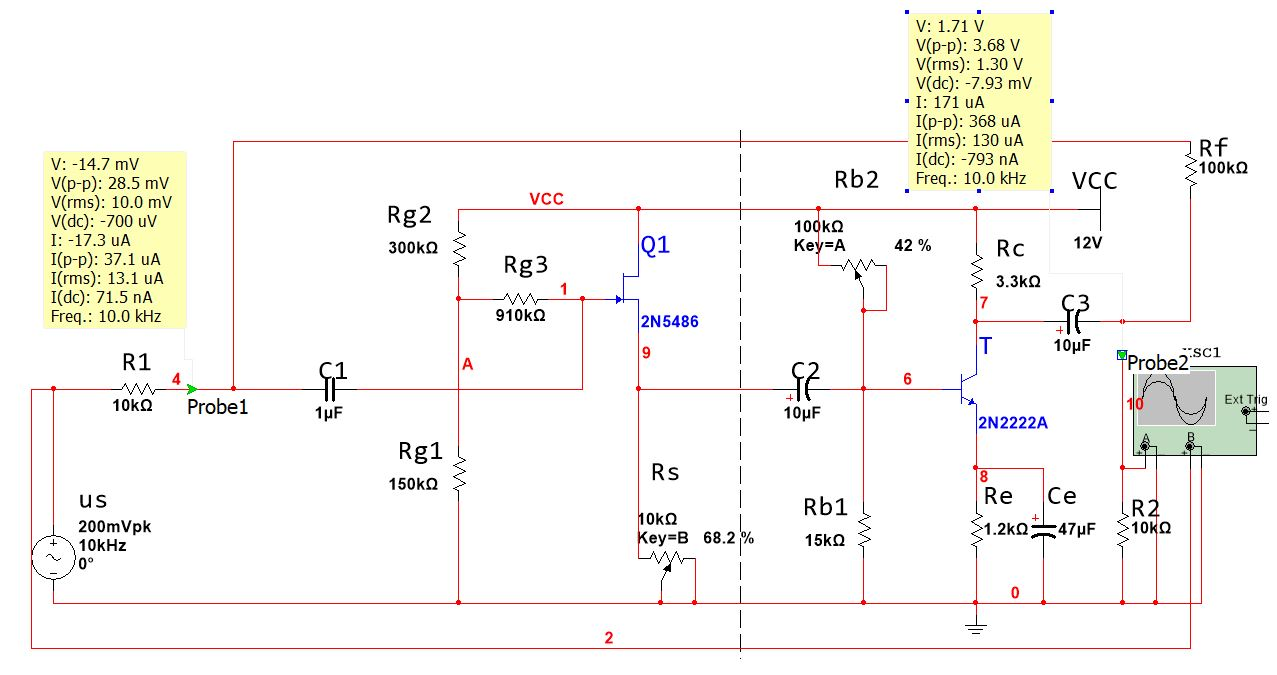
\includegraphics[width=\textwidth]{R.jpg}
\caption{输入输出电阻测试图}
\label{R}
\end{figure}

\begin{figure}
\centering
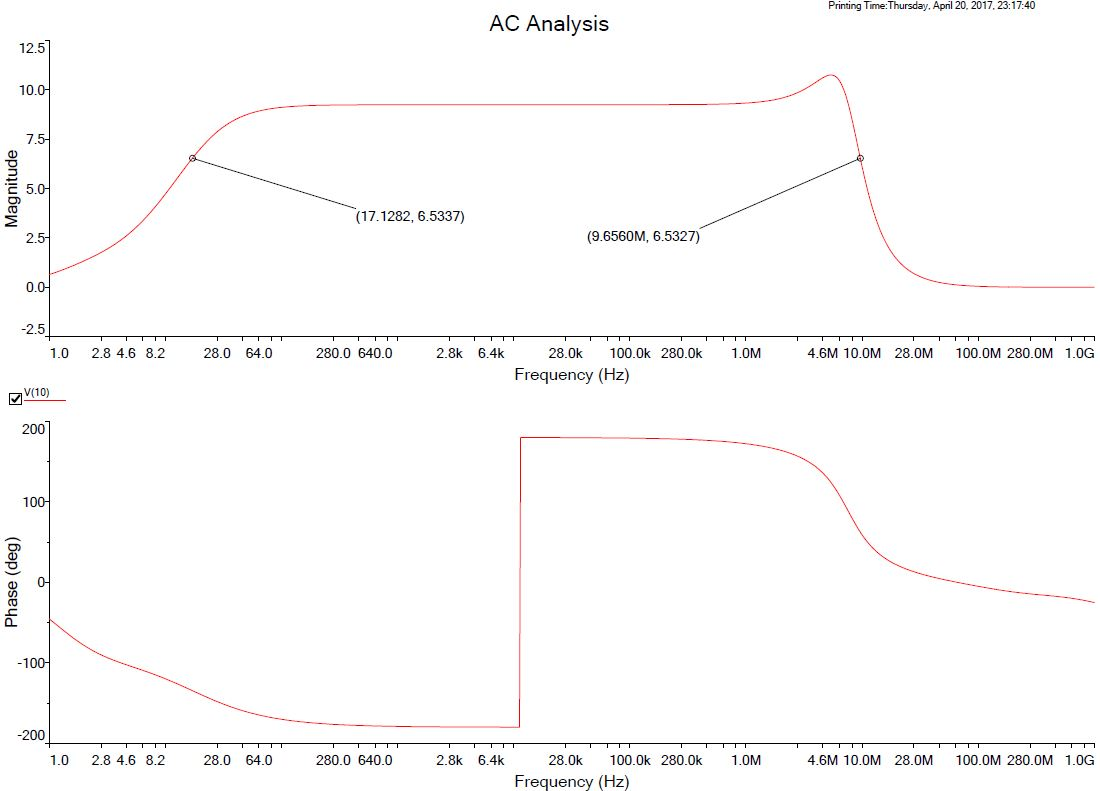
\includegraphics[width=\textwidth]{F.jpg}
\caption{辐频响应特性图}
\label{F}
\end{figure}

\section{电流并联负反馈的电路理论估计}
\subsection{仿真分析}
因为电路之中的参数计算大部分已经在上几次实验中完成,重新计算大同小异,而且存在着比较大的误差,因此这里用仿真进行测量。
\subsubsection{静态工作点测量}
按照题目中的要求搭建电路如图\ref{Q2}所示,首先对电路的静态工作点进行测量,得到$I_{CQ}=2.09\mathrm{mA},I_{DQ}=1.95\mathrm{mA}$,同时得到$U_{GDQ}=-4\mathrm{V},U_{CEQ}=3\mathrm{V}$满足题目中给定的要求.
\subsubsection{动态工作特性测量}
如图\ref{A2}所示测量电路的动态放大特性,得到负载开路的时候电路的动态放大倍数为$$A_{usf}=\frac{1885.3+1877.1\mathrm{mV}}{400\mathrm{mV}}=9.406$$

进一步通过探针测量电路的输入输出电阻,如图\ref{R2}所示,可以得到电路的输入电阻为
$$R_{if}=\frac{36.6\mathrm{mV}}{120\mu\mathrm{A}}=305\Omega$$
同时,在负载端加$5.0\mathrm{k}\Omega$的电阻,测量输出电压峰峰值为2.25V,因此得到输出电阻为
$$R_{of}=\frac{1885.3+1877.1-2250\mathrm{mV}}{449\mu\mathrm{A}}=3.36\mathrm{k}\Omega$$可以看出电路并非在深度饱和状态工作。
\begin{figure}
\centering
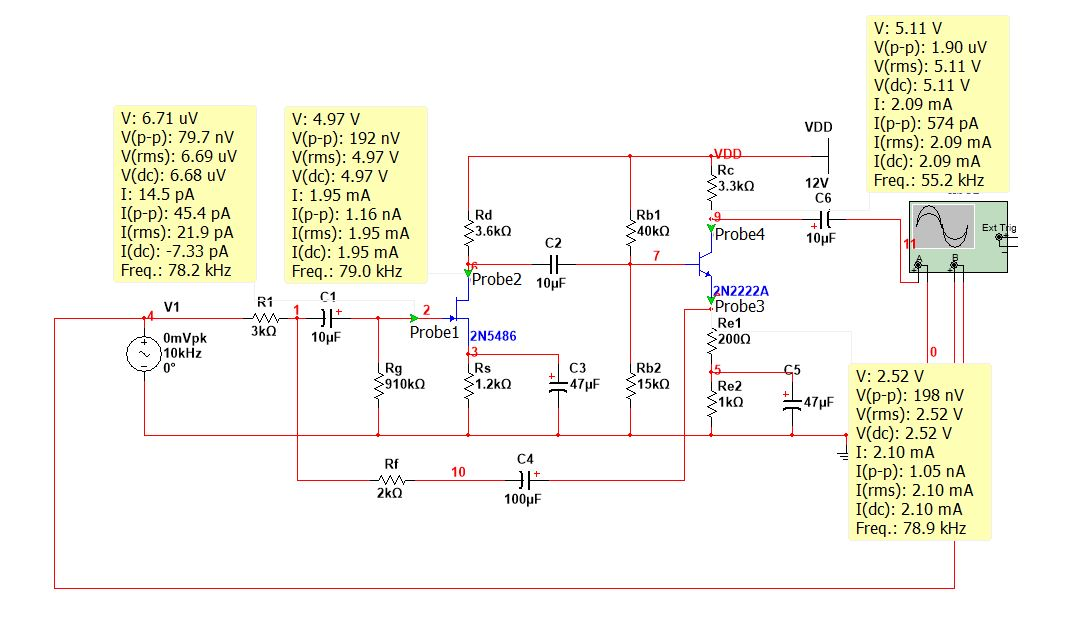
\includegraphics[width=\textwidth]{Q2.jpg}
\caption{电路图和静态工作点的测量}
\label{Q2}
\end{figure}
\begin{figure}
\centering
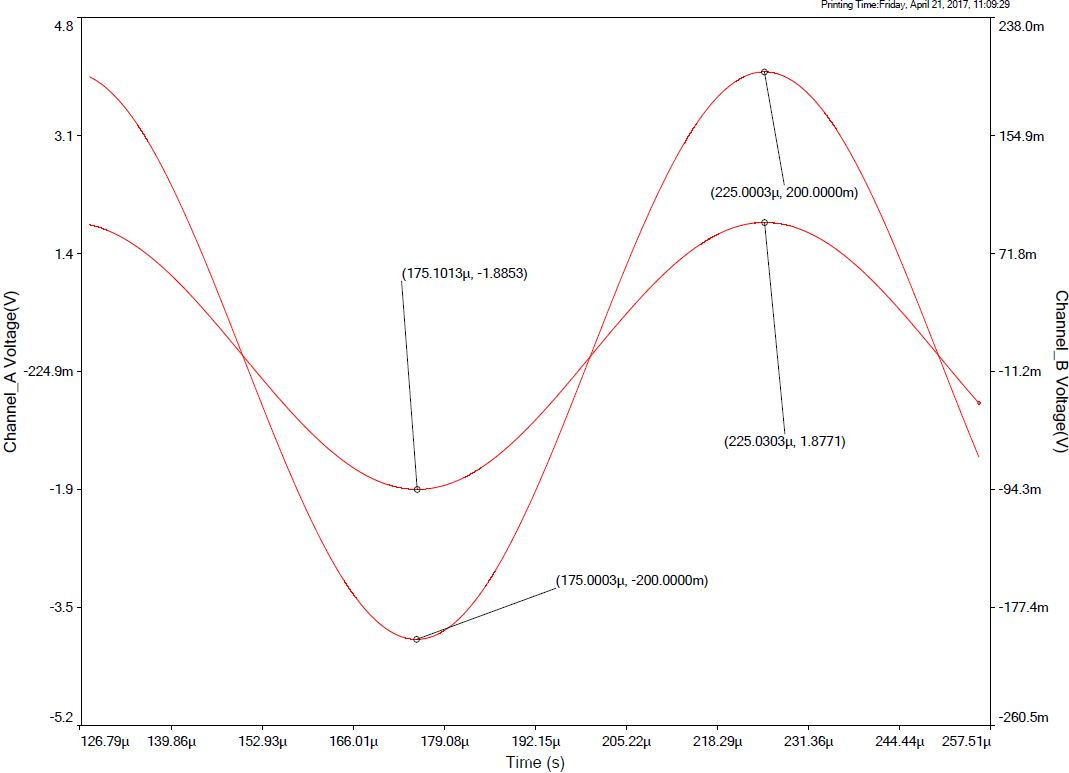
\includegraphics[width=\textwidth]{A2.jpg}
\caption{负载开路时输出电压放大倍数的测试}
\label{A2}
\end{figure}
\begin{figure}
\centering
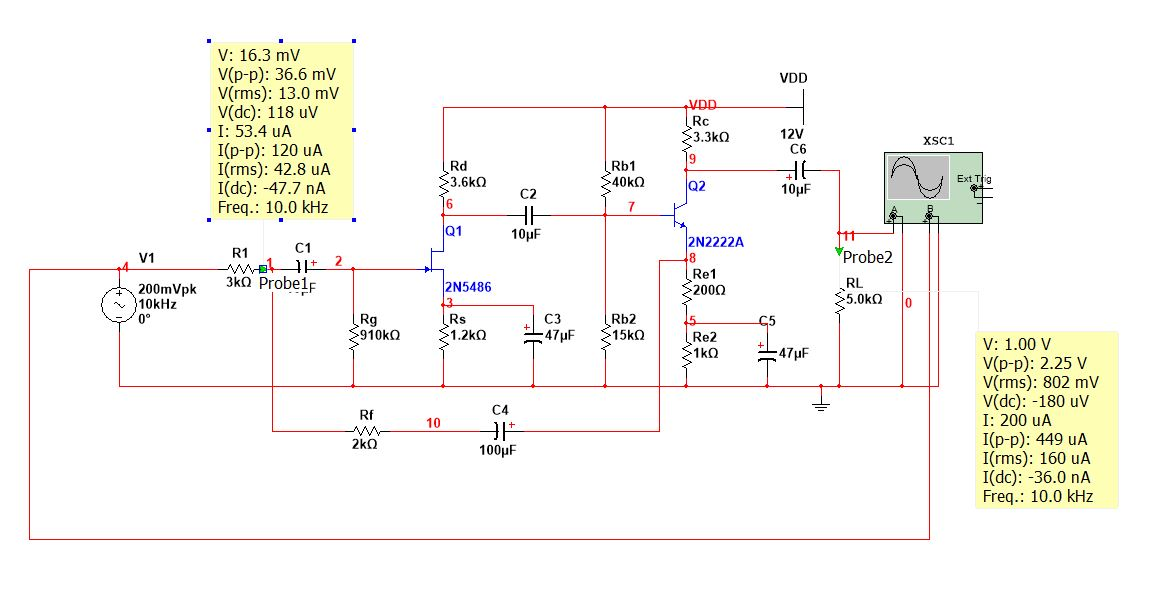
\includegraphics[width=\textwidth]{R2.jpg}
\caption{输入输出电阻的测量}
\label{R2}
\end{figure}
\clearpage
\section{实验数据分析}
\subsection{必做任务}
\subsubsection{放大倍数的测量}
实验采用$V_{pp}=400\mathrm{mV}$的输入电压对电路特性进行测量,得到输出电压峰值为1.91V和1.92V,计算可以得到电路的电压放大倍数为-9.6V/V,设计参数-10,相对误差4\%可以接受。

\begin{figure}
\centering
\includegraphics[width=\textwidth]{scope_0.bmp}
\caption{必做实验不带负载输出电压波形图}
\end{figure}

\subsubsection{输入电阻的测量}
下面进行输入电阻的测量,输入电压$V_{pk}=200\rm{mV}$,如图\ref{R}所示,信号源电阻$R_1$右侧电压上下两峰分别为14.1mV,13.2mV,可以计算得到
$$R_{ifs}=10\mathrm{k}\Omega\frac{14.1+13.2}{400}=730\Omega$$理论计算$R_{ifs}=768\Omega$,相对误差可以接受

\begin{figure}
\centering
\includegraphics[width=\textwidth]{scope_1.bmp}
\caption{信号源电阻$R_1$右侧电压}
\end{figure}

\subsubsection{输出电阻的测量}
输出电阻的测量:保持输入电压不变,原负载开路输出电压峰峰值为3.83V,负载接入$R_L=1\mathrm{k}\Omega$电阻,输出电压峰峰值变为3.2V,因此可以计算输出电阻为
$$R_{osf}=1\mathrm{k}\Omega\frac{3.83-3.2}{3.2}=187\Omega$$
理论计算$R_o=147\Omega$,相对误差可以忽略不计。

\begin{figure}
\centering
\includegraphics[width=\textwidth]{scope_3.bmp}
\caption{负载接入$R_L=1\mathrm{k}\Omega$电阻,输出电压峰峰值}
\end{figure}

\subsubsection{高低频率特性的测量}
实验测量高频特性和低频特性,得到$F_L=20\mathrm{Hz},F_H=1\mathrm{MHz}$,可以看出频带得到了展宽

\subsection{选做任务}
\subsubsection{放大倍数的测量}
实验采用$V_{pp}=400\mathrm{mV}$的输入电压对电路特性进行测量,得到输出电压峰值为1.8V和1.8V,计算可以得到电路的电压放大倍数为9.0V/V。
\subsubsection{输入电阻的测量}
下面进行输入电阻的测量,输入电压$V_{pk}=200\rm{mV}$,如图\ref{R2}所示,信号源电阻$R_1$右侧电压峰峰值为44.75mV可以计算得到
$$R_{ifs}=3\mathrm{k}\Omega\frac{44.75}{355.25}=379\Omega$$理论计算$R_{ifs}=305\Omega$,相对误差可以接受
\subsubsection{输出电阻的测量}
输出电阻的测量:保持输入电压不变,原负载开路输出电压峰峰值为3.83V,负载接入$R_L=1\mathrm{k}\Omega$电阻,输出电压峰峰值变为835mV,因此可以计算输出电阻为
$$R_{osf}=1\mathrm{k}\Omega\frac{835\mathrm{mV}}{2.765\mathrm{V}}=3.31\mathrm{k}\Omega$$
理论计算$R_o=3.36\mathrm{k}\Omega$,相对误差可以忽略不计。
\section{数据分析和实验总结}
\subsection{实验测量方法介绍}
输出电压放大倍数直接采用示波器贯彻,输入输出电阻采用串联电阻分压法测量,其中输入电阻的分压电阻由电压源内阻代替,输出电阻的分压由串联负载电阻处理。
\subsection{误差分析}
主要的误差在于实验元件技术相关参数测量值和理论值存在差异,同时在近似计算反馈性能时采用了深度负反馈条件,而实际上的反馈深度可能带来近似误差。另外存在如接线电阻等其他干扰。

总体上来说,实验的误差在5\%的量级以下。
\subsection{实验中问题}
本次电路搭建较为顺利,先通过逐级测试放大电路回复开环放大电路,在开环稳定后闭环,很快得到了准确的结果。

\subsection{负反馈对电路性能的影响}
引入负反馈会降低电路的放大倍数,但能使其较稳定,同时,引入负反馈也会影响输入输出电阻和幅频
特性:引入串联负反馈使输入电阻增大,引入并联负反馈使输入电阻减小,引入电压负反馈使输出电阻减小,
引入电流负反馈使输出电阻增大。由仿真实验和理论分析也可知引入负反馈可以一定程度上展宽电路的通频
带。理论计算时采取的交流等效模型及深度负反馈的计算方法可能会与实验值有一定的差异。
\end{document}
